\documentclass[10pt,a4paper]{article}
\usepackage[margin=27mm]{geometry}
\usepackage{fontspec}
\usepackage{amsmath,amsthm,amssymb,mathtools}
\usepackage{unicode-math}
\setmainfont{TeX Gyre Pagella}
\setsansfont{TeX Gyre Heros}
\setmonofont{DejaVu Sans Mono}[Scale=MatchLowercase]
\setmathfont{Asana Math}
\setmathfont{Latin Modern Math}[range={\lrcorner,\triangleleft,\triangleright}]
\usepackage{esint,booktabs,longtable,array,multirow,calc}
\usepackage{graphicx,xcolor,enumitem,hyperref,bookmark,alphalph}
\hypersetup{colorlinks=true,linkcolor=blue!40!black,citecolor=blue!40!black,urlcolor=blue!40!black,hypertexnames=false}
\usepackage{tikz}
\usetikzlibrary{arrows.meta,positioning}
\newtheorem{theorem}{Theorem}[section]
\newtheorem{proposition}[theorem]{Proposition}
\newtheorem{lemma}[theorem]{Lemma}
\newtheorem{corollary}[theorem]{Corollary}
\theoremstyle{definition}
\newtheorem{definition}[theorem]{Definition}
\newtheorem{problem}[theorem]{Problem}
\theoremstyle{remark}
\newtheorem{remark}[theorem]{Remark}
\numberwithin{equation}{section}
\providecommand{\Ric}{\operatorname{Ric}}
\providecommand{\Rm}{\operatorname{Rm}}
\providecommand{\Vol}{\operatorname{Vol}}
\providecommand{\E}{\mathcal E}
\providecommand{\J}{\mathcal J}
\providecommand{\tr}{\operatorname{tr}}
\providecommand{\supp}{\operatorname{supp}}
\providecommand{\diam}{\operatorname{diam}}
\providecommand{\dist}{\operatorname{dist}}
\providecommand{\Id}{\operatorname{Id}}
\providecommand{\Scal}{\operatorname{Scal}}
\providecommand{\Spin}{\operatorname{Spin}}
\providecommand{\HS}{\mathrm{HS}}
\providecommand{\TT}{\mathrm{TT}}
\providecommand{\dvol}{\,d\mu}
\providecommand{\dd}{\,d\mu_g}
\providecommand{\R}{\mathbb R}
\providecommand{\Z}{\mathbb Z}
\providecommand{\CP}{\mathbb{CP}}
\providecommand{\op}{\mathrm{op}}
\providecommand{\Dcal}{\mathcal D}
\providecommand{\av}{\fint}
\providecommand{\avgint}{\fint}
\providecommand{\norm}[1]{\left\lVert#1\right\rVert}
\providecommand{\spec}{\operatorname{Spec}}
\providecommand{\Met}{\operatorname{Met}}
\providecommand{\owedge}{\mathbin{\bigcirc\mkern-15mu\wedge}}
\newtheorem{target}[theorem]{Conditional extension}
\usepackage{tabularx,xurl}
\makeatletter
\renewcommand*\l@section{\@dottedtocline{1}{1.5em}{3.1em}}
\makeatother
\newcolumntype{L}[1]{>{\raggedright\arraybackslash}p{#1}}
\providecommand{\tightlist}{\setlength{\itemsep}{0pt}\setlength{\parskip}{0pt}}
\providecommand{\pandocbounded}[1]{#1}
\setlength{\emergencystretch}{3em}
\setlength{\parskip}{3pt}
\allowdisplaybreaks
\setcounter{tocdepth}{1}
\title{Integral Einstein Rigidity and the Geometry of Monopole Defects}
\author{}
\date{}
\begin{document}
\maketitle
\begin{abstract}
We study the differential compatibility of curvature and actual monopole
fields on closed oriented four-manifolds. A bounded field determines a
polynomial Weyl model. Covariant Hessian identities and a weak Bianchi
self-test turn incompatibility with this model into an integral Einstein
obstruction without an a priori compactness hypothesis. A constant-weight
formulation requires a single monopole solution on a negative Yamabe
representative. At a distinguished parameter it gives a trace-free Ricci
gap, with an explicit cost for negative class square. A finer argument
retains a non-small curvature background annihilating the calibrated
spinor and controls scalar slack by trace-free Ricci energy and the
scalar--Weyl deficit. The resulting two-chirality inequality has linear
topological scale, matched by actual surgery constructions. We develop
the associated variational reductions, period constraints, signed
characteristic identities, marked filling costs, and controlled geometric
realization results. The unrestricted weak zero-Weyl endpoint and the
optimal first-order coefficient for the balanced surgery family are
formulated separately from the theorems proved here.
\end{abstract}
\tableofcontents
\clearpage
\section{Introduction}
\label{sec:introduction}

An algebraically admissible curvature tensor need not be realizable by a
metric satisfying a prescribed differential equation. In four dimensions
the discrepancy is particularly visible when a monopole field selects a
self-dual direction. The scalar, Weyl, and Ricci components must then
satisfy not only Chern--Weil and monopole inequalities but also the field
equations, the connection identities, and the differential Bianchi
identity for the same metric. Our purpose is to measure this discrepancy
in integral norms, including regimes in which geometric compactness has
not been assumed.

The distinction between an unattainable equality and a positive distance
from equality is essential. An equality classification alone cannot
exclude degenerating sequences. The analysis below instead produces a
smooth test field and estimates the same divergence energy in two ways.
The field is constructed from an actual solution; in particular, it is
not a choice of eigenvectors across a multiple eigenvalue. Its Hessian
is controlled by integration by parts, rather than by a uniform Sobolev
inequality. The classical monopole curvature inequalities and their
equality geometry remain indispensable inputs
\cite{LeBrun2001,Kotschick2004,IshidaLeBrun2003,IMN2016}.

\subsection{The principal quantities}
Throughout, unless stated otherwise, $M$ is a closed connected oriented
smooth four-manifold. Put
\[
 \begin{gathered}
 T_\pm=2\chi(M)\pm3\tau(M),\quad T=T_+,\quad V=\Vol_g(M),\\
 P=\int_M|\Ric_g^\circ|^2,\quad S=\int_Ms_g^2,
 \quad R=\int_M|\Ric_g|^2=P+\frac14S.
 \end{gathered}
\]
Ricci curvature has its tensor norm. Weyl curvature has the
Hilbert--Schmidt norm as an endomorphism of $\Lambda^\pm$; two-forms have
their exterior-algebra norm. Thus
\begin{equation}\label{eq:intro-cw}
 4\pi^2T=\frac{S}{24}+2\int_M|W^+|^2-\frac{P}{2}.
\end{equation}
For a determinant class $a=c_1(L)$, write $p=(a_g^+)^2$ and assume, when
specified, a positive projection budget $p\ge A>0$. The two normalized
Einstein defects are
\begin{equation}\label{eq:intro-defects}
 \E(g)=\inf_{\lambda\ne0}
 \frac{\int_M|\Ric_g-\lambda g|^2}{\lambda^2V},
 \qquad \J(g)=\frac{4P}{R}\quad(R>0).
\end{equation}
The first quantity tests proximity to a nonzero Einstein multiple after
constant rescaling; the second measures the trace-free fraction of Ricci
energy. The exact relation is
\[
 \E(g)=4-\frac{(\int_Ms_g)^2}{VR}
       =\J(g)+\frac{S-(\int_Ms_g)^2/V}{R}.
\]
In particular $\J\le\E$, with equality at constant scalar curvature.
At a Ricci-flat metric $\J$ is undefined and $\E=4$; positive projection
budgets for actual monopoles exclude that case by the field equation, not by this
quotient.

\subsection{The common analytical mechanism}
For $\beta\ge2$ define
\[
 D_\beta=\left(1+\frac1\beta\right)S
       +6(\beta+1)\int_M|W^+|^2-72\pi^2p.
\]
The relevant actual solvability hypotheses make $D_\beta$ nonnegative.
On a representative with $s=-4$, one ordinary monopole solution, rescaled
to $F_A^+=2i\sigma(\Phi)$, suffices for the finite-parameter estimate
\begin{equation}\label{eq:intro-parameter}
 (1+b)\left(r+\frac{D_\beta}{\beta V}\right)
 \ge c_{\rm par}\frac{(\beta-2)^2}{\beta^4},
 \qquad r=\frac{P}{V},\quad b=\frac{(-a^2)_+}{V}.
\end{equation}
The hypotheses and complete field calculation appear in
Section~\ref{sec:single-parameter}. The endpoint $\beta=2$ is an actual
Kähler--Einstein equality branch; the estimate is not a prohibition of
that branch.

At $\beta=8$ the coefficients align with \eqref{eq:intro-cw}:
\[
 D_8=108\pi^2\left(T-\frac23p\right)+\frac{27}{2}P.
\]
Combining this identity with the exact conformal transfer yields
\begin{equation}\label{eq:intro-n1}
 \J(g)+\left(\frac TA-\frac23\right)_+
 \ge\frac{c_*}{1+(-a^2)_+/(2\pi^2A)}.
\end{equation}
Here the negative Yamabe representative of $[g]$ must possess the same
actual single solution with $p\ge A$. A companion inequality is
$\J(g)+(T/A-2/3)_+\ge c/(1+(T-a^2)_+/A)$. In particular the
cost in \eqref{eq:intro-n1} vanishes when $a^2\ge0$, including the
range $0\le a^2<T$. A positive lower bound for $\J$ itself is obtained
precisely when the topological summand is smaller than the displayed
right-hand side. Section~\ref{sec:tracefree-gap} proves these statements,
including their conformal and finite-cover quantifiers.

A second mechanism becomes available at the Kähler calibration. Let
\[
 \Sigma=S-32\pi^2p,\qquad \Pi=P+D_2,
 \qquad Y=(T-a^2)_+.
\]
Under actual conformal monopole supply,
\begin{equation}\label{eq:intro-linear}
 \Sigma\le C\bigl(\Pi+\sqrt{\Pi Y}\bigr).
\end{equation}
This is an all-metric estimate without an additional scalar-variance
term. Its proof does not charge the whole background curvature to the
error. It retains an algebraic curvature model whose action annihilates
the distinguished spinor, absorbs the remaining determinant energy by
the class-square identity, and closes the same-field Bianchi test.
Section~\ref{sec:linear-coercivity} supplies this argument.

If $a^2\ge T$, set
\[
 h=1-\frac TA\in(0,1/3],\qquad
 U=\frac{3\min(T_+,T_-)}{A}.
\]
Combining \eqref{eq:intro-linear} with the two chiral Chern--Weil
identities gives
\begin{equation}\label{eq:intro-window}
 \J(g)+(U-1-h)_+\ge ch.
\end{equation}
This linear scale is realized on a balanced family of blowups and
handle additions to complex-hyperbolic covers:
\[
 c_1h_j\le\inf_g\J(g)=\inf_g\E(g)
      \le\frac{4h_j}{1+h_j},\qquad h_j\longrightarrow0.
\]
The lower bound, actual gauge supply, and recovery construction concern
the same smooth manifolds. The optimal balanced coefficient is not
asserted to be $4$. The handle-only subfamily has an exact infimum.

\subsection{Geometry beyond the obstruction}
The later sections retain the geometric information not summarized by
\eqref{eq:intro-n1}--\eqref{eq:intro-window}. Simultaneous actual
fields impose positive-inertia and sign-correlation constraints on
period matrices. On compatible branches, saturation can supply smooth
forms and force bidisk or complex-hyperbolic geometry under specified
global hypotheses. Integral identities on marked fillings separate
whole-core cost from terminal bubble cost. Actual local torsion models
show why determinant charge alone does not control torsion index.
Signed transgression and curvature-action identities keep track of the
remaining interactions without assuming their sign.

The logical distinction is mathematical: a coercive inequality, an
optimal energy value, a description of minimizing sequences, and an
existence theorem are different conclusions. The proofs below use
additional hypotheses only where the relevant conclusion requires them.
In particular, no implication from vanishing obstruction to unrestricted
Einstein existence is used.

Fixed-exterior equality geometry supplies a complementary description
of the allowed boundary. Section~\ref{sec:early-equality-geometry}
identifies ordinary monopole classes under the marked cohomological
hypotheses, retains all terms in the Hodge--volume identity, and follows
the first-order equations into the radial bubble-period argument.
Its evaluation-injectivity hypothesis is stated where the final volume
separation requires it. The local-development, slow-mode, and filling
arguments similarly retain their geometric hypotheses rather than
being subsumed into an unrestricted compactness assertion.

For comparison with pointwise approximation, set
\[
 \delta_\sigma(g)=\|g^{-1}\Ric_g-\sigma\Id\|_{L^\infty,\mathrm{op}},
 \qquad \sigma\in\{-1,1\}.
\]
The pointwise existence question asks whether a sufficiently small
dimension-dependent value of this quantity forces the same smooth
manifold to admit some Einstein metric. The output is not required to
be close to the input, to retain its auxiliary structures, or to have
the same Einstein constant. In dimension four, $\E(g)\le4\delta_\sigma(g)^2$.
Our integral obstructions and controlled realization theorems address
specified actual-input classes; the fixed-bundle constructions explain
why failure of a local repair does not decide the unrestricted existence
question.

\subsection{Classical inputs and comparison}
Ordinary monopole classes, special monopole classes, stable-cohomotopy
supply, and twisted double-cover supply enter through their actual
solvability statements. They are not replaced by a formal cohomology
vector. The classical results of LeBrun, Kotschick, Ishida--LeBrun, and
Ishida--Matsuo--Nakamura provide these distinct inputs and the comparison
inequalities. In the matching positive-budget ranges the integral
conclusions strengthen the corresponding exact Einstein obstructions.
The comparison with a specified set of supplied classes is distinguished
from optimization over all monopole classes of the same manifold.

The complete proofs are organized by mathematical dependence. The
intrinsic calibration and weighted pencil precede their constant-weight
refinement; the coercivity and variational theorems then feed the
geometric constructions. The supplements contain the further structure,
filling, and realization arguments used to delimit these results.
\begin{figure}[ht]
\centering
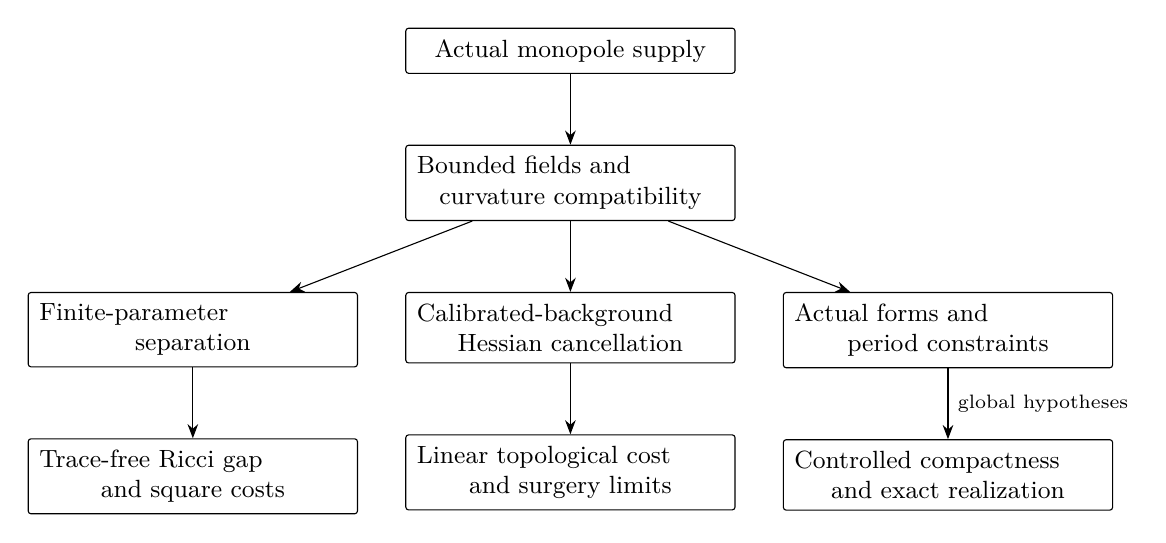
\begin{tikzpicture}[
 node distance=9mm and 6mm,
 box/.style={draw,rounded corners=1pt,align=center,font=\small,
             text width=39mm,inner sep=4pt},
 arr/.style={-{Stealth[length=1.8mm]}}]
\node[box] (supply) {Actual monopole supply};
\node[box,below=of supply] (field) {Bounded fields and\newline curvature compatibility};
\node[box,below left=of field] (parameter) {Finite-parameter\newline separation};
\node[box,below=of field] (linear) {Calibrated-background\newline Hessian cancellation};
\node[box,below right=of field] (forms) {Actual forms and\newline period constraints};
\node[box,below=of parameter] (gap) {Trace-free Ricci gap\newline and square costs};
\node[box,below=of linear] (cost) {Linear topological cost\newline and surgery limits};
\node[box,below=of forms] (real) {Controlled compactness\newline and exact realization};
\draw[arr] (supply)--(field);
\draw[arr] (field)--(parameter);
\draw[arr] (field)--(linear);
\draw[arr] (field)--(forms);
\draw[arr] (parameter)--(gap);
\draw[arr] (linear)--(cost);
\draw[arr] (forms)--node[right,font=\scriptsize]{global hypotheses}(real);
\end{tikzpicture}
\caption{The principal proof dependencies. The realization arrow includes
the global hypotheses stated in the corresponding theorems; it is not
a converse to the obstruction inequalities.}
\end{figure}
\clearpage
